\nonstopmode
\documentclass{beamer}
\def\part{1}
\usepackage{listings}
\usepackage{fancyvrb}

\usepackage{pgf}
\usepackage[english]{babel}
\usepackage[latin1]{inputenc}
\usepackage{times}
\mode<article>
{
  \usepackage{times}
  \usepackage{mathptmx}
  \usepackage[left=1.5cm,right=6cm,top=1.5cm,bottom=3cm]{geometry}
}

\usepackage{hyperref}
\usepackage[T1]{fontenc}
\usepackage{tikz}
\usepackage{colortbl}
%\usepackage{yfonts}
%\usepackage{colortbl}
%\usepackage{translator} % comment this, if not available


% Common settings for all lectures in this course

\def\lecturename{BEAST II 101}

\title{\insertlecture}

\author{Remco Bouckaert}

\institute
{
  Auckland University\\
  New Zealand
}

\subject{Vorlesung \lecturename}




% Beamer version theme settings

\useoutertheme[height=0pt,width=2cm,right]{sidebar}
\usecolortheme{rose,sidebartab}
\useinnertheme{circles}
\usefonttheme[only large]{structurebold}

\setbeamercolor{sidebar right}{bg=black!15}
\setbeamercolor{structure}{fg=blue}
\setbeamercolor{author}{parent=structure}

\setbeamerfont{title}{series=\normalfont,size=\LARGE}
\setbeamerfont{title in sidebar}{series=\bfseries}
\setbeamerfont{author in sidebar}{series=\bfseries}
\setbeamerfont*{item}{series=}
\setbeamerfont{frametitle}{size=}
\setbeamerfont{block title}{size=\small}
\setbeamerfont{subtitle}{size=\normalsize,series=\normalfont}

\setbeamertemplate{navigation symbols}{}
\setbeamertemplate{bibliography item}[book]
\setbeamertemplate{sidebar right}
{
  {\usebeamerfont{title in sidebar}%
    \vskip1.5em%
    \hskip3pt%
    \usebeamercolor[fg]{title in sidebar}%
    \insertshorttitle[width=2cm,center,respectlinebreaks]\par%
    \vskip1.25em%
  }%
  {%
    \hskip3pt%
    \usebeamercolor[fg]{author in sidebar}%
    \usebeamerfont{author in sidebar}%
    \insertshortauthor[width=2cm,center,respectlinebreaks]\par%
    \vskip1.25em%
  }%
  \hbox to2cm{\hss\insertlogo\hss}
  \vskip1.25em%
  \insertverticalnavigation{2cm}%
  \vfill
  \hbox to 2cm{\hfill\usebeamerfont{subsection in
      sidebar}\strut\usebeamercolor[fg]{subsection in
      sidebar}%\insertshortlecture.
      \insertframenumber\hskip5pt}%
  \vskip3pt%
}%

\setbeamertemplate{title page}
{
  \vbox{}
  \vskip1em
 % {\huge \insertshortlecture\par}
  {\usebeamercolor[fg]{title}\usebeamerfont{title}\inserttitle\par}%
  \ifx\insertsubtitle\@empty%
  \else%
    \vskip0.25em%
    {\usebeamerfont{subtitle}\usebeamercolor[fg]{subtitle}\insertsubtitle\par}%
  \fi%     
  \vskip1em\par
  %Vorlesung \emph{\lecturename}\ vom \insertdate\par
  \vskip0pt plus1filll
  \leftskip=0pt plus1fill\insertauthor\par
  \insertinstitute\vskip1em
}

\logo{
\includegraphics[width=1cm]{auckland.png}}



% Article version layout settings

\mode<article>

\makeatletter
\def\@listI{\leftmargin\leftmargini
  \parsep 0pt
  \topsep 5\p@   \@plus3\p@ \@minus5\p@
  \itemsep0pt}
\let\@listi=\@listI


\setbeamertemplate{frametitle}{\paragraph*{\insertframetitle\
    \ \small\insertframesubtitle}\ \par
}
\setbeamertemplate{frame end}{%
  \marginpar{\scriptsize\hbox to 1cm{\sffamily%
      \hfill\strut%\insertshortlecture.
    \insertframenumber}\hrule height .2pt}}
\setlength{\marginparwidth}{1cm}
\setlength{\marginparsep}{4.5cm}




\let\origstartsection=\@startsection
\def\@startsection#1#2#3#4#5#6{%
  \origstartsection{#1}{#2}{#3}{#4}{#5}{#6\normalfont\sffamily\color{blue!50!black}\selectfont}}

\makeatother

\mode
<all>




% Typesetting Listings

\usepackage{listings}
\lstset{language=Java,XML}

\alt<presentation>
{\lstset{%
%  basicstyle=\footnotesize\ttfamily,
  basicstyle=\scriptsize\ttfamily,
  commentstyle=\slshape\color{blue!50!black},
  keywordstyle=\bfseries\color{blue!50!black},
  identifierstyle=\color{blue},
  stringstyle=\color{orange},
  escapechar=\#,
  emphstyle=\color{red}}
}
{
  \lstset{%
    basicstyle=\ttfamily,
    keywordstyle=\bfseries,
    commentstyle=\itshape,
    escapechar=\#,
    emphstyle=\bfseries\color{red}
  }
}



% Common theorem-like environments

\theoremstyle{definition}
\newtheorem{exercise}[theorem]{\translate{Exercise}}




% New useful definitions:

\newbox\mytempbox
\newdimen\mytempdimen

\newcommand\includegraphicscopyright[3][]{%
  \leavevmode\vbox{\vskip3pt\raggedright\setbox\mytempbox=\hbox{\includegraphics[#1]{#2}}%
    \mytempdimen=\wd\mytempbox\box\mytempbox\par\vskip1pt%
    \fontsize{3}{3.5}\selectfont{\color{black!25}{\vbox{\hsize=\mytempdimen#3}}}\vskip3pt%
}}

\newenvironment{colortabular}[1]{\medskip\rowcolors[]{1}{blue!20}{blue!10}\tabular{#1}\rowcolor{blue!40}}{\endtabular\medskip}

\def\equad{\leavevmode\hbox{}\quad}

\newenvironment{bluecolortabular}[1]
{\medskip\rowcolors[]{1}{blue!50!black!20}{blue!50!black!10}%
  \tabular{#1}\rowcolor{blue!50!black!40}}%
{\endtabular\medskip}


%\mode<presentation>
%{
%  \usetheme{PaloAlto}
%  \usetheme{Bergen}
  %\usetheme{Berkeley}
  %\setbeamercovered{transparent}
%}


\usepackage[english]{babel}
\usepackage[latin1]{inputenc}
\usepackage{times}
\usepackage[T1]{fontenc}







\if \part 1
\title[Beast II 101]{Beast II 101: Part 1\\ 
\includegraphics{../../src/beast/app/draw/icons/beast.png}}
\fi
\if \part 2
\title[Beast II 101]{Beast II 101: Part 2\\ 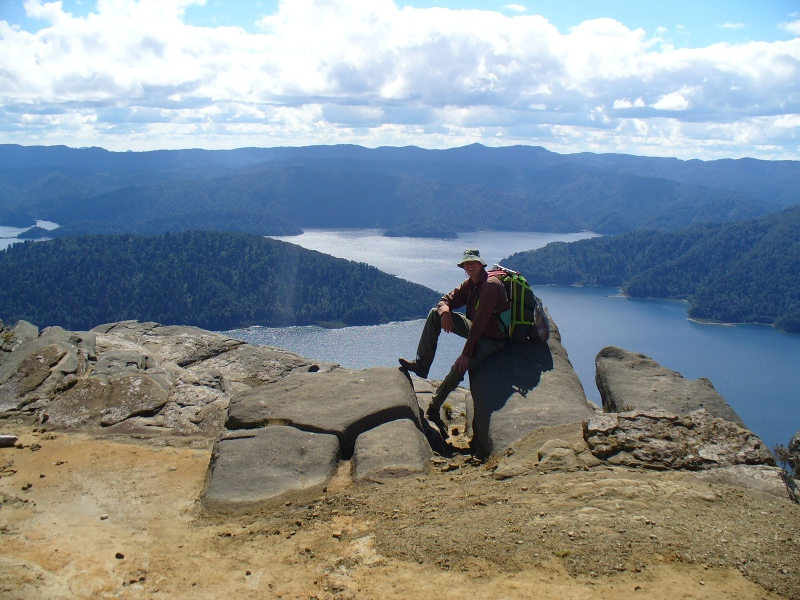
\includegraphics[width=0.75\textwidth]{walk.jpg}}
\fi
\if \part 3
\title[Beast II 101]{Beast II 101: Part 3\\ 
\includegraphics{../../src/beast/app/draw/icons/beast.png}}
\fi

%\subtitle{}

\author[Bouckaert] 
{Remco R. Bouckaert\\\url{remco@cs.{auckland|waikato}.ac.nz}}

\institute[University of Auckland|Waikato]
{Department of Computer Science\\
  University of Auckland \& University of Waikato
}
\date[] % (optional)
{}

\subject{Beast II 101}


% If you wish to uncover everything in a step-wise fashion, uncomment
% the following command: 

%\beamerdefaultoverlayspecification{<+->}


\begin{document}
\begin{frame}
  \titlepage




%done: likelihood should check alignment, check frequencies
%done: validate tree in likelihood covers all taxa
%done: getters and setters
%done: fix BeagleTest
%done: fix random branch rate model
%
%done: test all taxa in alignment are unique
%done: test all taxa in tree are unique
%done: taxon id -> name (beware impact on BEAUti)
%done: ambiguous characters + custom data types 
%done: sync SNAP
%done: robustify StateNodes
%done: set up beastii
%done: check validation rules on all inputs
%done: ambiguous in TreeLikelihood
%done: clean up likelihood files
%TODO: port more substitution models
%TODO: write test cases
%TODO: add-on distribution mechanism
%TODO: finish BEAUti
\end{frame}

\if \part 1


\section{BEAST 2 basics}


\begin{frame}{Jukes Cantor}
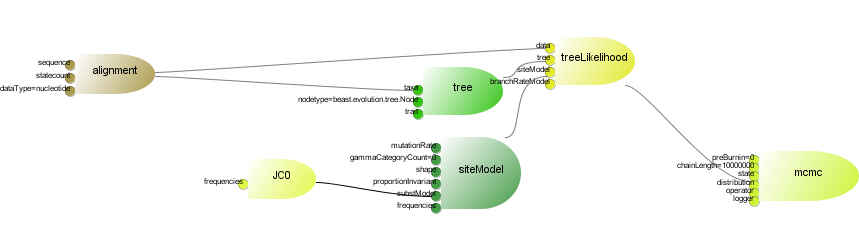
\includegraphics[width=\textwidth]{example1.png}

All objects are Plugins - connected to each other through Inputs
\end{frame}
\begin{frame}{HKY}
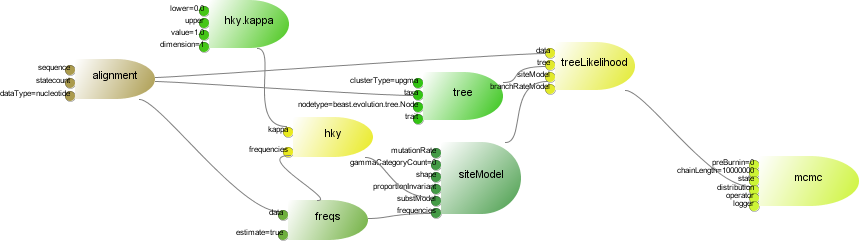
\includegraphics[width=\textwidth]{example2.png}

Adding kappa parameter and frequencies
\end{frame}
\begin{frame}{Adding operators}
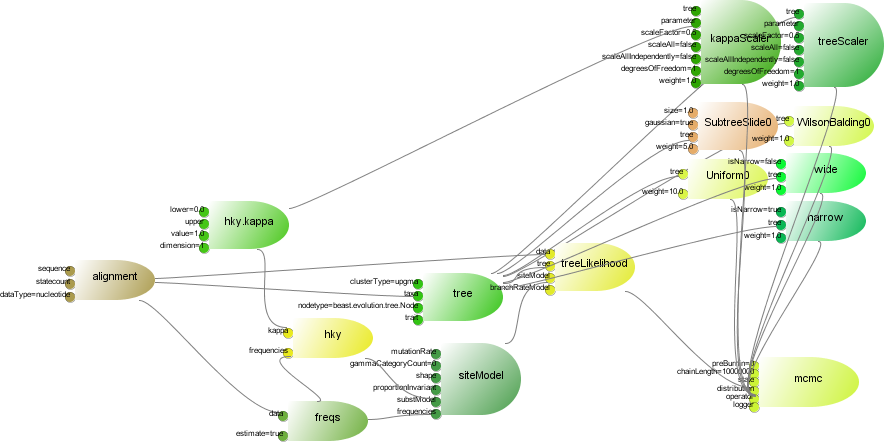
\includegraphics[width=\textwidth]{example3.png}

Operate on kappa parameter and tree
\end{frame}
\begin{frame}{Adding State}
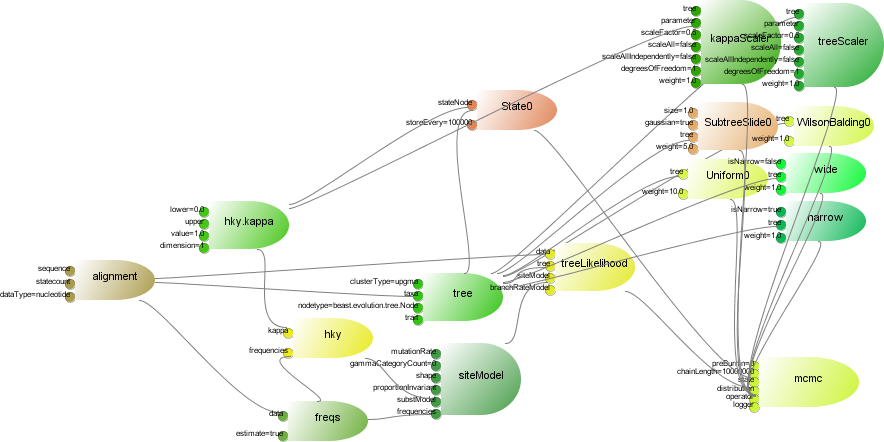
\includegraphics[width=\textwidth]{example4.png}

The state contains every Plugin that operators work on
\end{frame}
\begin{frame}{Adding Loggers}
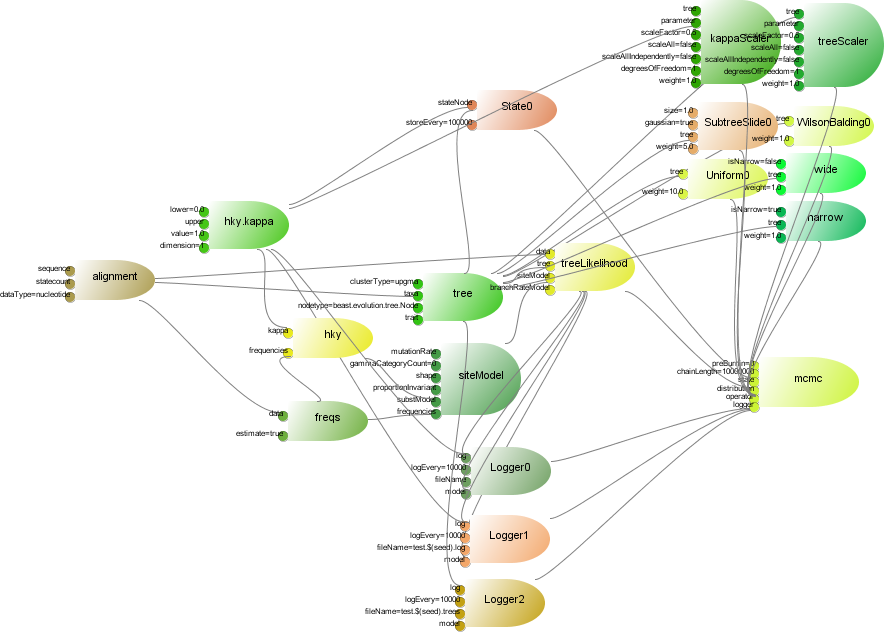
\includegraphics[width=\textwidth]{example5.png}

3 loggers: screen, trace and trees
\end{frame}
\begin{frame}{Adding Sequences}
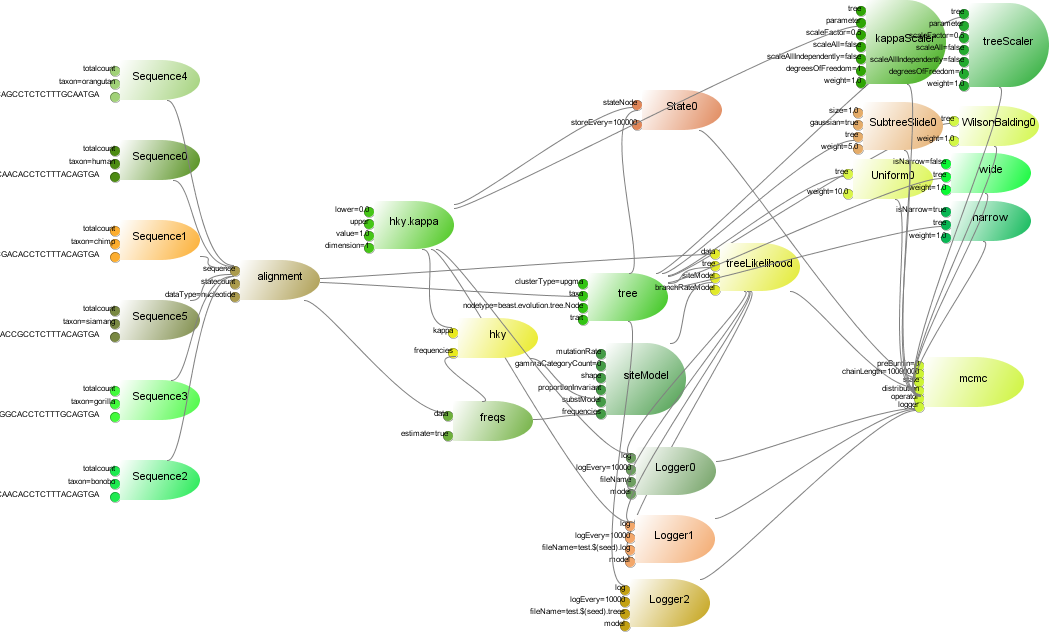
\includegraphics[width=\textwidth]{example6.png}

Inputs to alignments, which takes care of the patterns, DataType and set of Taxon names
\end{frame}


\begin{frame}{What BEAST 2 does}
...supposed to do...

\begin{itemize}
\item The kind of Bayesian analysis as per citations on the BEAST 1 wiki.
\item BEAUti 2: GUI to specify analysis.
\item Provide a platform to develop add-ons - powerful interface, easy extensible XML, templates for BEAUti.
\item Sequence generator for simulation studies.
\item Documentation for all the above -- from user to developer, XML tweaker, etc.
\end{itemize}

\end{frame}

\begin{frame}{What BEAST 2 doesn't}
\begin{itemize}
\item Post-analysis processing like Tracer, tree annotator, tree log analyser, DensiTree, KML producer
\item Most non-Bayesian analysis
\item Laundry
\end{itemize}

\end{frame}


\subsection{Plugins}

\begin{frame}[containsverbatim]
{Phylosophy}

Everything is a plug-in
\vskip0.5cm
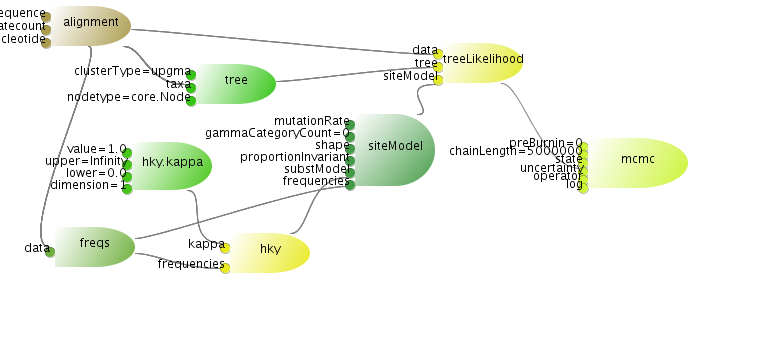
\includegraphics[width=\textwidth]{hkymodel.png}

Plug-ins provide...
\begin{itemize}
\item connection with with other plug-ins/values through 'inputs'
\item validation
\item documentation
\item 'XML parsing'
\end{itemize}
\end{frame}

\begin{frame}[containsverbatim]
{Plugin class}

\begin{lstlisting}[language=java]
@Description("Description goes here")
public class Plugin {
    public void initAndValidate()

    public String getDescription()
    public String getCitations()

    public String getID()
    public void setID(String sID)

} // class Plugin
\end{lstlisting}

\end{frame}

\begin{frame}[containsverbatim]
{A minimal plugin}

{\color{blue}\begin{lstlisting}[language=java]
@Description("Description of MyPlugin goes here")
public class MyPlugin extends Plugin {
    public Input<Integer> value = new Input<Integer>("value",
        "value used by my plugin");

    public void initAndValidate() throws Exception {
        // go check stuff and 
        // do stuff that normally goes in a constructor
    }

} // class MyPlugin
\end{lstlisting}}
\end{frame}


\begin{frame}[containsverbatim]
{HKY Plugin}

{
%\lstset{basicstyle=\small}
\tiny
\begin{lstlisting}[language=java]
@Description("HKY85 (Hasegawa, Kishino & Yano, 1985) substitution model of nucleotide evolution.")
@Citation("Hasegawa, M., Kishino, H and Yano, T. 1985. Dating the human-ape splitting by a molecular clock of mitochondrial DNA. " +
        "Journal of Molecular Evolution 22:160-174.")
public class HKY extends 'Plugin' {
    public Input<Frequencies> freqs = new Input<Frequencies>("frequencies", "frequencies nucleotide letters");
    public Input<Parameter> kappa = new Input<Parameter>("kappa", "kappa parameter in HKY model", Validate.REQUIRED);

    @Override public void initAndValidate() throws Exception {
        initialiseEigen();        
    }

     public void getTransitionProbabilities(Node node, 
      		double fStartTime, 
		double fEndTime, 
		double fRate, 
		double[] matrix) {...}
 
    @Override
    protected boolean requiresRecalculation() {...}

    @Override public void store() {...}
    @Override public void restore() {... }
} // class HKY
\end{lstlisting}
}
\end{frame}

\subsection{Inputs}

\begin{frame}[containsverbatim]
{Inputs}
\pgfputat{\pgfxy(5,-1)}{\pgfbox[left,base]{\pgfimage[width=5cm]{hkymodel.png}}}
Simple primitives

\begin{lstlisting}[language=java]
public Input<Boolean> scaleAll = 
    new Input<Boolean>("scaleAll", 
        "if true, all elements of a parameter are scaled, otherwise one is randomly selected");
\end{lstlisting}

Other plugins

\begin{lstlisting}[language=java]
public Input<Frequencies> freqs = 
    new Input<Frequencies>("frequencies", 
        "frequencies of nucleotide letters");
\end{lstlisting}

Multiple inputs

\begin{lstlisting}[language=java]
public Input<List<Parameter>> parameters = 
    new Input<List<Parameter>>("parameter", 
        "parameter, part of the state",
        new ArrayList<Parameter>());
\end{lstlisting}
\end{frame}

\begin{frame}[containsverbatim]
{Inputs}

Enumerations

\begin{lstlisting}[language=java]
final static String [] UNITS =  {"year", "month", "day"};

public Input<String> units = new Input<String>("units", 
        "name of the units in which values are posed, " +
		"used for conversion to a real value. This can be " + 
        Arrays.toString(UNITS) + " (default 'year')", 
        "year", 
        UNITS);
\end{lstlisting}
\end{frame}

\begin{frame}[containsverbatim]
{Input validation}

Default: OPTIONAL (see previous slide)
\vskip0.2cm
If input is REQUIRED:

\begin{lstlisting}[language=java]
public Input<Parameter> kappa = 
    new Input<Parameter>("kappa", 
        "kappa parameter in HKY model",
        Validate.REQUIRED);
\end{lstlisting}

\begin{lstlisting}[language=java]
public Input<List<Operator>> operators = 
    new Input<List<Operator>>("operator",
        "operator for generating proposals in MCMC state space",
        new ArrayList<Operator>(), Validate.REQUIRED);
\end{lstlisting}

If input is XOR:

\begin{lstlisting}[language=java]
public Input<Tree> tree = 
    new Input<Tree>("tree", 
        "if specified, all tree branch length are scaled");
public Input<Parameter> parameter = 
    new Input<Parameter>("parameter", 
        "if specified, this parameter is scaled"
        , Validate.XOR, tree);
\end{lstlisting}

\end{frame}


\section{MCMC library}


\begin{frame}[containsverbatim]
{State}
\begin{itemize}
\item State is explicit in XML \& as object (unlike BEAST 1)
\item Contains StateNodes, e.g., parameters and trees
\item Operators work on the StateNodes
\begin{lstlisting}[language=java]
public double proposal() throws Exception {...}
\end{lstlisting}
%\item Log probability calculated given state
%\begin{lstlisting}[language=java]
%public double calculateLogP() throws Exception {...}
%\end{lstlisting}
%\item State can be interrogated on value of parameters/trees
%\begin{lstlisting}[language=java]
%state.getParameter(/**Parameter**/ p)
%state.getTree(/**Tree**/ t)
%\end{lstlisting}
\item State can be stored to disk/restored
\item State can store/restore itself for MCMC proposals
\end{itemize}
\end{frame}


\begin{frame}{MCMC Library}

StateNode vs CalculationNode

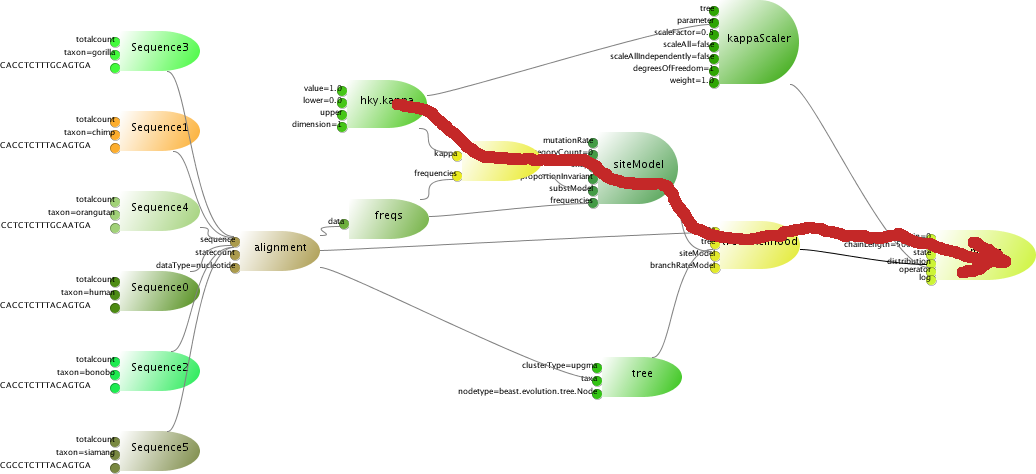
\includegraphics[width=\textwidth]{hky.png}

\end{frame}


\begin{frame}[containsverbatim]{Plugin hierarchy}
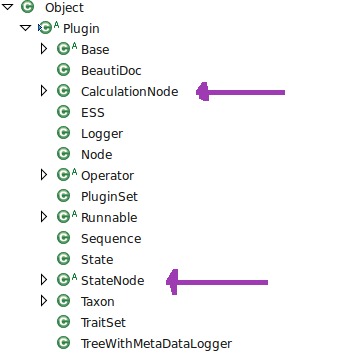
\includegraphics{hierarchy1.png}
Just parameters and trees
\end{frame}

\begin{frame}[containsverbatim]{StateNode hierarchy}
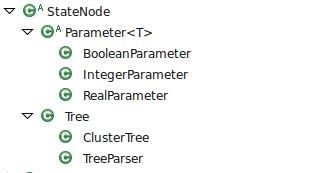
\includegraphics[width=\textwidth]{hierarchy3.png}
\end{frame}

\begin{frame}[containsverbatim]{CalculationNode hierarchy}
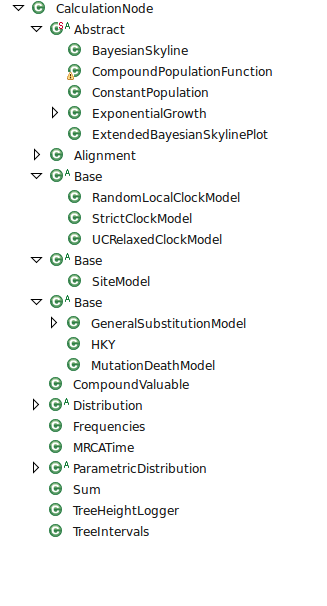
\includegraphics[width=0.5\textwidth]{hierarchy2.png}
\end{frame}


\subsection{Loop}

\begin{frame}
{MCMC loop 
\only<2>{effect on\\ state nodes}
\only<3>{effect on\\ calculation nodes}
\only<4>{\\CalculationNode method calls}}
\pgfputat{\pgfxy(6,-1)}{\pgfbox[left,base]{\pgfimage[width=6cm]{hky.png}}}

\begin{itemize}
\item[] \only<2-4>{\color{green}Store state}
\item[] \color{black}Propose new state
\item[] \only<3-4>{\color{blue}store calculation nodes} \only<4>{\color{red} store()}
\item[] \only<3-4>{\color{blue}check dirtyness} \only<3>{calculation nodes} \only<4>{\color{red} requiresRecalculation()}
\item[] \color{black}logP = calculateLogP();
\item[] \color{black}if (new state is acceptable) 
\item[] \mbox{\hskip1cm}\only<1>{// do something}\only<2-4>{\color{green}accept state} 
\item[] \only<3-4>{\mbox{\hskip1cm}\color{blue}mark calculation nodes clean} \only<4>{\color{red} accept()}
\item[] \color{black}else
\item[] \mbox{\hskip1cm}\only<1>{// do something else}\only<2-4>{\color{green}restore state}
\item[] \only<3-4>{\mbox{\hskip1cm}\color{blue}restore calculation nodes} \only<4>{\color{red} restore()}
\item[] \only<2-4>{\color{green}mark state clean}
\end{itemize}
\end{frame}

\subsection{Classes}

\begin{frame}{BEAST class structure}
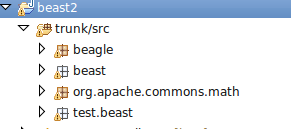
\includegraphics[width=0.7\textwidth]{classes1.png}

beast - main beast classes

beagle and apache libraries

test - for junit tests

\end{frame}

\begin{frame}{BEAST core class structure}
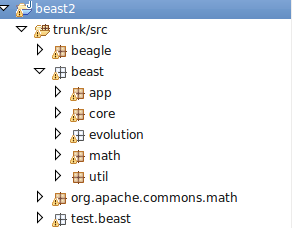
\includegraphics[width=0.7\textwidth]{classes2.png}

app - applications like BeastMCMC, BEAUti, SequenceGenerator

core, evolution - MCMC and evolution libraries

math - mathematical classes

util - utilities like parsers, XML producers, random nr generator, class discovery.

\end{frame}

\begin{frame}{BEAST core class structure}
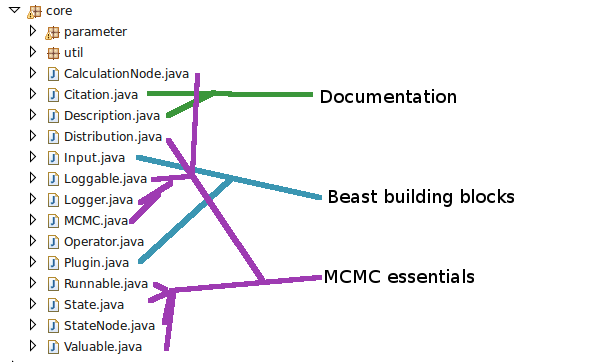
\includegraphics[width=\textwidth]{classes3.png}
\end{frame}

\begin{frame}{BEAST core class structure}
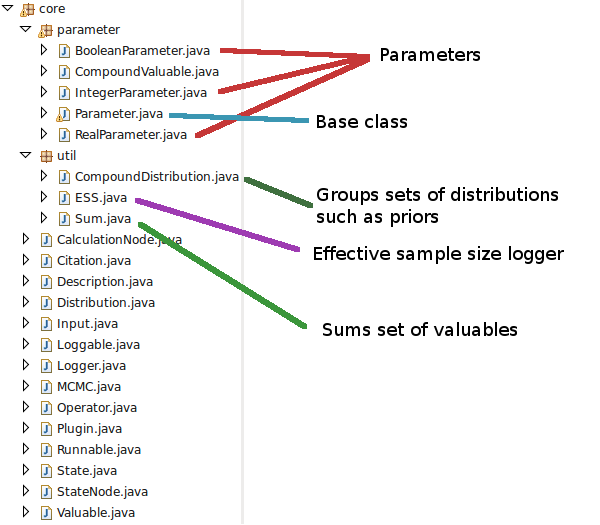
\includegraphics[width=\textwidth]{classes4.png}
\end{frame}


\section{Evolution library}

\begin{frame}[containsverbatim]{Evolution packages}
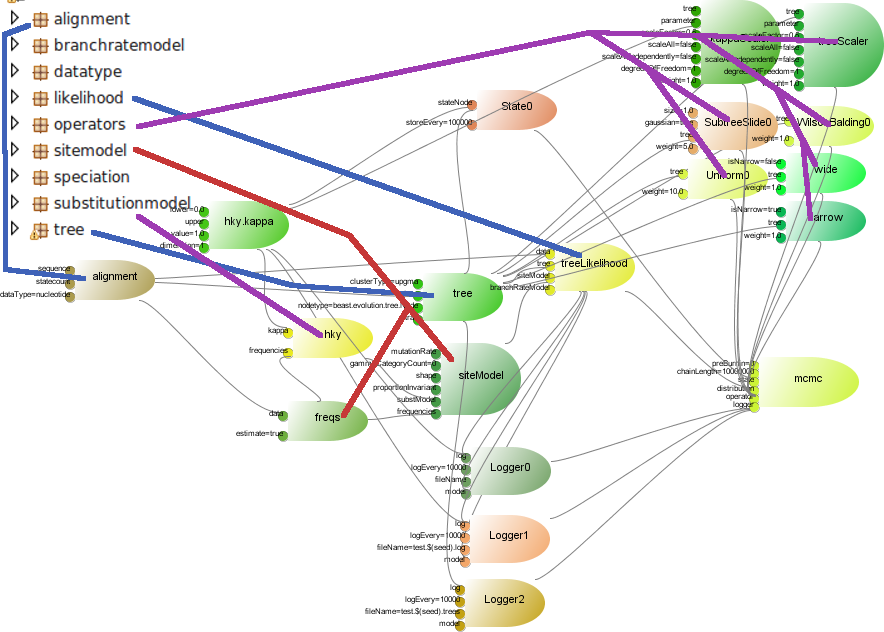
\includegraphics[width=\textwidth]{classes5b.png}

Important classes you might want to derive from: SubstitutionModel, Operator, 
BranchRateModel, Coalescent, SpeciationLikelihood, (DataType, Alignment,
SiteModel).
\end{frame}

\begin{frame}[containsverbatim]{Evolution - alignment classes}
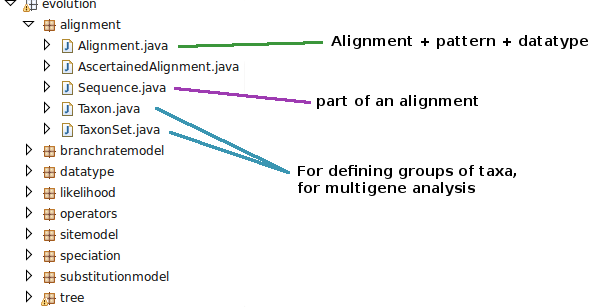
\includegraphics[width=\textwidth]{classes6.png}
\end{frame}

\begin{frame}[containsverbatim]{Evolution - branch rate model classes}
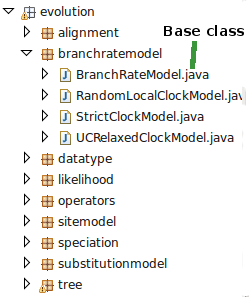
\includegraphics{classes7.png}
\end{frame}

\begin{frame}[containsverbatim]{Evolution - data type classes}
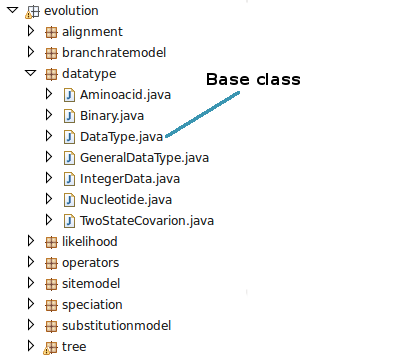
\includegraphics[width=\textwidth]{classes8.png}
\end{frame}

\begin{frame}[containsverbatim]{Evolution - operator classes}
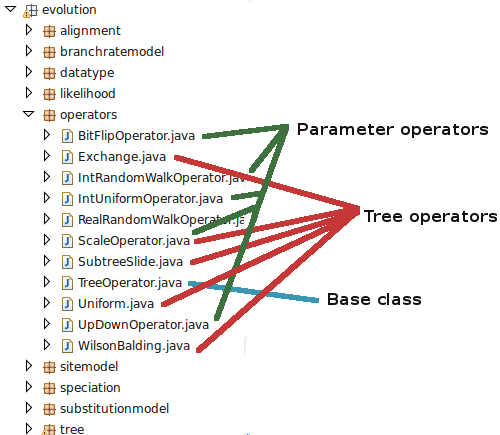
\includegraphics[width=\textwidth]{classes9.png}
\end{frame}


\begin{frame}[containsverbatim]{Evolution - site model classes}
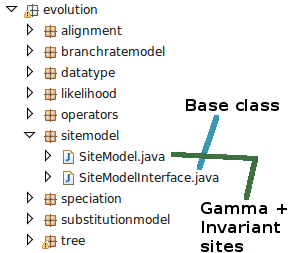
\includegraphics{classes10.png}
\end{frame}

\begin{frame}[containsverbatim]{Evolution - speciation classes}
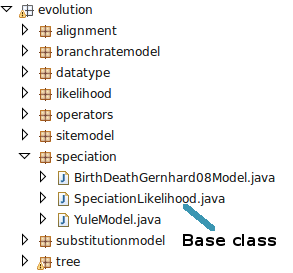
\includegraphics{classes11.png}
\end{frame}

\begin{frame}[containsverbatim]{Utility classes}
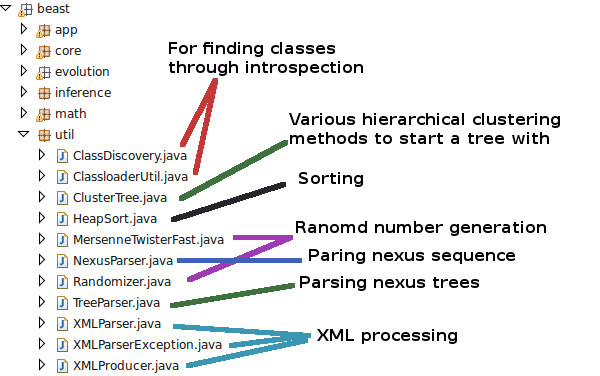
\includegraphics[width=\textwidth]{classes12.png}
\end{frame}




\section{Design patterns}

\begin{frame}[containsverbatim]{Variable naming}

{\small In case you wondered where those funny names came from...}\vskip0.5cm

Variable name format: {\tt$<$scope$> <$type$> <$name$>$}

scope 
\begin{itemize}
\item {\tt m\_} prefix for member variables
\item {\tt g\_} globals = static member variables
\item none otherwise
\end{itemize}

type
\begin{itemize}
\item {\tt s} string
\item {\tt f} floating point number (double or float)
\item {\tt n} number
\item {\tt i} indicator
\item {\tt b} boolean
\item {\tt p} pointer to object
\end{itemize}


\end{frame}

\begin{frame}[containsverbatim]{Basic plugin layout}

\begin{lstlisting}[language=java]
@Description("Some sensible description of the Plugin")
public class MyPlugin extends Plugin {
    <!-- inputs first -->
    public Input<RealParamater> p = new Input<>...;

    <!-- members next -->
    private Object o;

    <!-- initAndValidate -->
    @Override
    public void initAndValidate() {...}

    <!-- class specific methods -->

    <!-- Overriding methods -->
}
\end{lstlisting}

\end{frame}


\begin{frame}[containsverbatim]{Accessing inputs {\em for reading, not writing!}}

Let there be an input:

\begin{lstlisting}[language=java]
public Input<RealParamater> p = new Input<>...;
\end{lstlisting}\vskip0.5cm

To get the parameter of input {\tt m\_p}, use\\ {\tt m\_p.get()}.\vskip0.5cm

To get the value of the parameter, use {\tt m\_p.get().getValue()}.\vskip0.5cm

Alternatively 

\begin{lstlisting}[language=java]
    RealParamater p = pInput.get();
    double fValue = p.getValue();
\end{lstlisting}

\end{frame}

\begin{frame}[containsverbatim]{requiresRecalculation()}

\begin{lstlisting}[language=java]
public boolean requiresRecalculation() {
	// for StateNode inputs only
	if (stateNodeInput.get().somethingIsDirty()) {
		return true;
	}

	// for CalculationNode inputs only
        if (calculationNodeInput.get().isDirtyCalculation()) {
		return true;
	}
	return false;
}
\end{lstlisting}

\end{frame}


\begin{frame}[containsverbatim]{Lean CalculationNode}


\begin{lstlisting}[language=java]
boolean needsUpdate; // flag to indicate internal state is up to date
public void initAndValidate() {needsUpdate = true;}
// CalculationNode specific interface that returns results
public Object calculateSomeThing() {
	if (needsUpdate) {
		update();
	}
	return someThing;
}
void update() {
	someThing = ...;
	needsUpdate = false;
}
public boolean requiresRecalculation() {
	if (someInputIsDirty()) {
		needsUpdate = true;
		return true;
	}
	return false;
}
public void store() {super.store();}
public void restore() {
	needsUpdate = true;
	super.restore();
}
\end{lstlisting}
\end{frame}

\begin{frame}[containsverbatim]{Fat CalculationNode}

As lean CalculationNode, but actually storing something

\begin{lstlisting}[language=java]
Object intermediateResult;
Object storedIntermediateResult;

public void initAndValidate() {
	// reserve space for result objects
	intermediateResult = new ...;
 	storedIntermediateResult = new ...;
}

public void store() {
	// copy intermediateResult to storedIntermediateResult
	...
	super.store();
}
public void restore() {
	// needsUpdate = true; <- don't need this now
	Object tmp = intermediateResult;
	intermediateResult = storedIntermediateResult;
	storedIntermediateResult = tmp;
	super.restore();
}
\end{lstlisting}

\end{frame}



\begin{frame}[containsverbatim]{Adding a Substitution model}
Extend SubstitutionModel.Base class

\begin{itemize}
\item A substitution model should implement {\tt getTransitionProbabilities(Node node, double fStartTime, double fEndTime, double fRate, double[] matrix)}
\item Typically, {\tt fRate * (fEndTime - fStartTime)} is the distance $t$ in $e^{Qt}$
and {\tt Node} can be ignored.
\item Results should go in the {\tt matrix}: note this is represented as array.
\item {\tt SubstitutionModel} is a {\tt CalculationNode}, so it may be worth implementing {\tt store/restore/requireRecalculation}
\end{itemize}

\end{frame}

\begin{frame}[containsverbatim]{Adding an Operator: Extend Operator class}

\begin{itemize}
\item An operator should have at least one input with a {\tt StateNode} to operate on.
\item An operator should implement {\tt proposal()} which changes the State.
\item {\tt proposal()} should return the Hastings ratio.
\item Return {\tt Double.NEGATIVE\_INFINITY} if the proposal is invalid/doomed
(don't throw Exceptions).
\item Implement {\tt optimize()} if auto-optimization applies.
%\item
%Note: use {\tt\bf \color{red}m\_parameter.get(this)} in {\tt proposal()} not {\tt \color{blue}m\_parameter.get()}
%{\bf iff you want to change the value of the {\tt StateNode}}
\end{itemize}


\end{frame}


\begin{frame}[containsverbatim]{Adding a logger: Implement Loggable interface}

\begin{lstlisting}[language=java]
    void init(PrintStream out) throws Exception;

    void log(int nSample, PrintStream out);

    void close(PrintStream out);
\end{lstlisting}

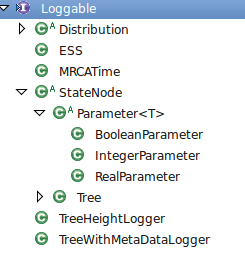
\includegraphics[widht=0.5\textwidth]{loggables.png}

\end{frame}



\if0
\begin{frame}[containsverbatim]{Shadowing inputs}

Never shadow a StateNode

\begin{lstlisting}[language=java]
    public Input<RealParamater> p = new Input<>...;
    private RealParameter pShadow;
\end{lstlisting}


Shadow CalculationNodes, 
primitives (Integer, Double, String, Boolen) inputs, 
and others is fine.


\begin{lstlisting}[language=java]
    public Input<Integer> p = new Input<>...;
    private Integer pShadow;
\end{lstlisting}


\end{frame}
\fi

\begin{frame}[containsverbatim]{Input rule of base class is not what you want.}

If an Input is REQUIRED for a base class you want to override, but for the derived
class this Input should be OPTIONAL, set the Input to OPTIONAL in the constructor.
E.g. for a SNPSequence that derives from Sequence, but for which m\_sData is optional,
add a constructor

{\color{blue}\begin{lstlisting}[language=java]
	public SNPSequence() {
		data.setRule(Validate.OPTIONAL);
	}
\end{lstlisting}}
Note that the constructor needs to be public, to prevent IllegalAccessExceptions
on construction by e.g. the XMLParser.

\end{frame}

\begin{frame}[containsverbatim]{Input parameter dimension is unknown...}

...but a CalculationNode can easily find out.\vskip 0.5cm

Then, in the {\tt initAndValidate()} method of the {\tt CalculationNode},
call {\tt parameter.setDimension(x)}


\end{frame}

\begin{frame}[containsverbatim]{Input parameter {\em value} is unknown...}

...but a CalculationNode can easily find out.\vskip 0.5cm

Then, in the {\tt initAndValidate()} method of the {\tt CalculationNode},
create a new Parameter X, and use {\tt input.get().assignFromWithoutID(X)}

\begin{lstlisting}[language=java]
@Override
public void initAndValidate() throws Exception {
    // determine dimension, number of Nodes in a tree here
	int nNodes = tree.get().getNodeCount();

    // create new Parameter
	IntegerParameter positions = new IntegerParameter("0", 0, Integer.MAX_VALUE, nNodes);
	for (int i = 0; i < nNodes; ++) {
		int iPosX = ...;
		positions.setValue(i, iPosX);
	}

    // copy values to the input
	positions.get().assignFromWithoutID(positions);
	
}
\end{lstlisting}

\end{frame}

\begin{frame}[containsverbatim]{Trees with traits}

For a tree with $n$ leaf nodes, so $2n-1$ nodes in total
\begin{itemize}
\item Easiest: associate a parameter with dimension $2n-1$ to the tree
\begin{itemize}
\item Leaf nodes are numbered $0,\ldots,n-1$
\item Internal nodes are numbered $n,\ldots,2n-1$
\item Root node is not treated as special internal node (no number guaranteed)
\end{itemize}
\item Harder: Derive from class {\tt Node} and process as meta-data
\end{itemize}

\end{frame}


\section{Ways to mess up}

\begin{frame}{Common errors}

1. {\bf\color{red} {\tt Input} is not declared public.}

If {\tt Input}s are not public, they cannot get values assigned by for
instance the {\tt XMLParser}.\vskip1cm

\pause

2. {\bf\color{red} Type of input is a template class (other than {\tt List}).}

Thanks to limitations of Java introspection and the way BEAST II is set up, Inputs should be 
of a type that is concrete, and apart from {\tt List<T>} no template class should be used.\vskip1cm

\pause
3. {\bf\color{red} Store/restore do not call {\tt super.store()}/{\tt super.restore()}.}

Obviously, not calling store/restore on super classes may result in unexpected behavior.

\end{frame}


\begin{frame}{Uncommon errors}
\begin{itemize}
\item Forgot to set {\tt m\_bNeedsUpdate} flag in {\tt requiresRecalculation()}. This way
the {\tt CalculationNode} will never update its internal state and will always return the
same (initially calculated) result.
\item always return {\tt false} from {\tt requiresRecalculation()}. This way {\tt CalculationNode}s 
downstream may never think of recalculating themselves.
\end{itemize}
Both issues will not be picked up during the debugging phase
of the MCMC loop.

\end{frame}


\fi
\if \part 2




\section{XML}

\begin{frame}{What is XML?}
"The Extensible Markup Language (XML) is a simple text-based format for representing structured information"\vskip1cm

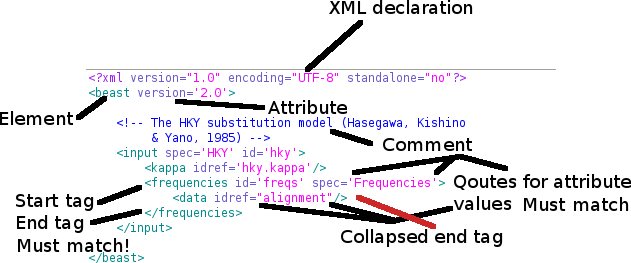
\includegraphics[width=\textwidth]{xml.png}\vskip1cm

{\small Reserved characters in attribute values: " (\&quot;) ' (\&apos;) $<$ (\&lt;) $>$ (\&gt;) \& (\&amp;)
e.g. x="\&quot;"}

\end{frame}


\begin{frame}{XML}
Let's put this model into XML 

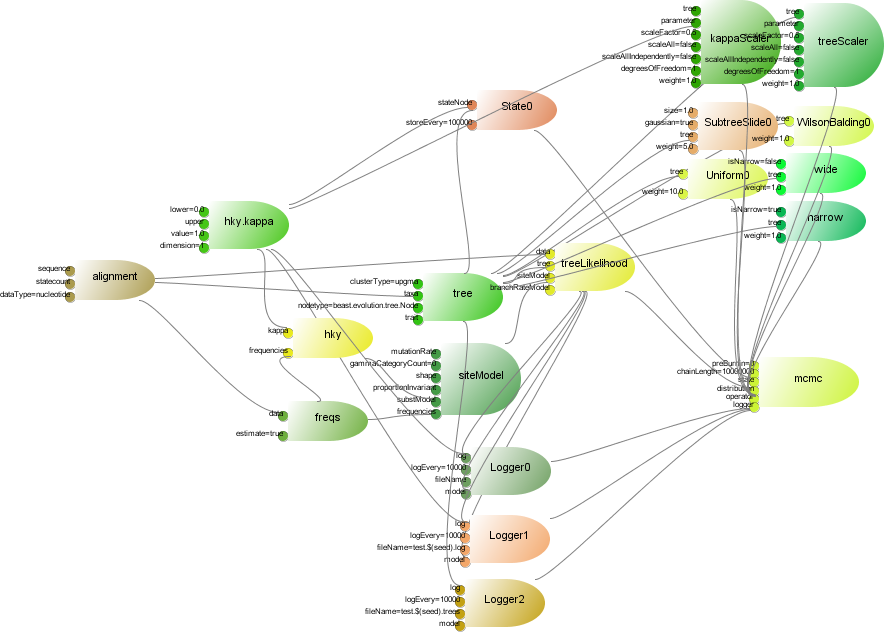
\includegraphics[width=\textwidth]{example5.png}

First the hky-scale operator

\end{frame}

\begin{frame}[containsverbatim]{BEAST 2 Reserved XML attributes}

{\tt name}, {\tt spec}, {\tt id}, {\tt idref}
\begin{itemize}
\item XML element {\tt input} can be used for every plugin.
\item Specify {\tt name} to match with input name.
\item Specify {\tt spec} to identity Plugin.
\item XML id/idref mechanism to reuse Plugins.
\item XML attributes for primitives (Integer, Double, Boolean, String).
\end{itemize}

{\small
\begin{lstlisting}[language=XML]
<input name='operator' id='kappaScaler' 
    spec='beast.evolution.operators.ScaleOperator' 
    scaleFactor='0.5' weight='1'>
    <input name='parameter' idref='hky.kappa'/>
</input>
\end{lstlisting}
}
\end{frame}

\begin{frame}[containsverbatim]{XML rule: namespaces}


Top level {\tt beast} element can be used to define namespaces
in the usual Java fashion.

\begin{lstlisting}[language=XML]
    <beast namespace="beast.core:beast.evolution.operators">
\end{lstlisting}

This allows shortening of spec-values:

{\small
\begin{lstlisting}[language=XML]
<input name='operator' id='kappaScaler' 
    spec='beast.evolution.operators.ScaleOperator' 
    scaleFactor='0.5' weight='1'>
    <input name='parameter' idref='hky.kappa'/>
</input>
\end{lstlisting}
}

becomes

{\small
\begin{lstlisting}[language=XML]
<input name='operator' id='kappaScaler' spec='ScaleOperator' 
    scaleFactor='0.5' weight='1'>
    <input name='parameter' idref='hky.kappa'/>
</input>
\end{lstlisting}
}
\end{frame}

\begin{frame}[containsverbatim]{XML rule: input/name}

Input elements with name attributes equal the name's value as element name

\begin{lstlisting}[language=XML]
<input name='xyz'></input>  == <xyz></xyz>
\end{lstlisting}

so

{\small
\begin{lstlisting}[language=XML]
<input name='operator' id='kappaScaler' spec='ScaleOperator' 
    scaleFactor='0.5' weight='1'>
    <input name='parameter' idref='hky.kappa'/>
</input>
\end{lstlisting}
}

equals

{\small
\begin{lstlisting}[language=XML]
<operator id='kappaScaler' spec='ScaleOperator' 
    scaleFactor='0.5' weight='1'>
    <parameter idref='hky.kappa'/>
</operator>
\end{lstlisting}
}
\end{frame}


\begin{frame}[containsverbatim]{XML rules: idref}

If idref is only attribute in element, an attribute with element
name and \@ before the idref.

\begin{lstlisting}[language=XML]
<name idref="some-id"/> == name='@some-id'
\end{lstlisting}

So

{\small
\begin{lstlisting}[language=XML]
<operator id='kappaScaler' spec='ScaleOperator' 
    scaleFactor='0.5' weight='1'>
    <parameter idref='hky.kappa'/>
</operator>
\end{lstlisting}
}

equals

{\small
\begin{lstlisting}[language=XML]
<operator id='kappaScaler' spec='ScaleOperator' 
    scaleFactor="0.5" weight="1" parameter="@hky.kappa"/>
\end{lstlisting}
}
\end{frame}


\begin{frame}[containsverbatim]{BEAST 2 Reserved XML elements}

{\small
%\pgfputat{\pgfxy(1.5,-4)}{\pgfbox[left,base]{\pgfimage[width=5cm]{BEAST.png}}}
\begin{Verbatim}[commandchars=\\\{\}]
\textcolor{blue}{\bf <beast} \textcolor{purple}{version=}\textcolor{black}{'2.0'} \textcolor{purple}{namespace=}\textcolor{black}{'x.y.z:a.b.c'}\textcolor{blue}{\bf >}
\textcolor{blue}{\bf <map} \textcolor{purple}{name=}\textcolor{black}{'xyz'}\textcolor{blue}{\bf >}x.y.z.Class\textcolor{blue}{\bf </map>}
element <xyz> is expanded to 
<input name='xyz' spec='x.y.z.Class'>

\textcolor{blue}{\bf <input}\textcolor{blue}{\bf >}

\textcolor{blue}{\bf <run}\textcolor{blue}{\bf >} spec must be beast.core.Runnable
\textcolor{blue}{\bf <distribution}\textcolor{blue}{\bf >} spec must be beast.core.Distribution
\textcolor{blue}{\bf <operator}\textcolor{blue}{\bf >} spec must be beast.core.Operator
\textcolor{blue}{\bf <logger}\textcolor{blue}{\bf >}    spec=beast.core.Logger
\textcolor{blue}{\bf <data}\textcolor{blue}{\bf >}      spec=beast.evolution.alignment.Alignment
\textcolor{blue}{\bf <sequence}\textcolor{blue}{\bf >}  spec=beast.evolution.alignment.Sequence
\textcolor{blue}{\bf <state}\textcolor{blue}{\bf >}     spec=beast.core.State
\textcolor{blue}{\bf <parameter}\textcolor{blue}{\bf >} spec=beast.core.parameter.RealParameter
\textcolor{blue}{\bf <tree}\textcolor{blue}{\bf >}      spec=beast.evolution.tree.Tree

\textcolor{blue}{\bf <plate}\textcolor{blue}{\bf >} mainly for BEAUti templates
\end{Verbatim}
}
\end{frame}



\begin{frame}[containsverbatim]{XML: example}

{\small

\begin{lstlisting}[language=XML]
<input name='substModel' id="hky" spec="HKY">
    <input name='kappa' idref="hky.kappa" >
    <input name='frequencies' id="freqs" spec="Frequencies">
           <input name='data' idref="alignment"/>
    </input>
</input>


<input spec="TreeLikelihood">
    <input name='data' idref='alignment'/>
    <input name='tree' idref='tree'/>
    <input name='siteModel' spec="SiteModel">
        <input name='substModel' idref='hky'/>
    </input>
</input>
\end{lstlisting}


\color{blue}Assuming {\tt namespace='beast.evolution.sitemodel:
beast.evolution.substitutionmodel:\
beast.evolution.likelihood'}
}
\end{frame}


\begin{frame}[containsverbatim]{Compress inputs}
Input elements with name attributes equal the name's value as element name

\begin{lstlisting}[language=XML]
<input name='xyz'></input>  == <xyz></xyz>
\end{lstlisting}

Applying to the example


{\small
\begin{lstlisting}[language=XML]
<substModel id="hky" spec="HKY">
    <kappa idref="hky.kappa" >
    <frequencies id="freqs" spec="Frequencies">
           <data idref="alignment"/>
    </frequencies>
</substModel>


<distribution spec="TreeLikelihood">
    <data idref='alignment'/>
    <tree idref='tree'/>
    <siteModel spec="SiteModel">
        <substModel idref='hky'/>
    </siteModel>
</distribution>
\end{lstlisting}
}
\end{frame}

\begin{frame}[containsverbatim]{Compress idrefs}

if idref is only attribute in element, an attribute with element
name and \@ before the idref.

\begin{lstlisting}[language=XML]
<name idref="some-id"/> == name='@some-id'
\end{lstlisting}

Applying to the example

{\small
\begin{lstlisting}[language=XML]

<substModel id="hky" spec="HKY" kappa="@hky.kappa" >
    <frequencies id="freqs" spec="Frequencies" 
        data="@alignment"/>
</substModel>

<distribution data="@alignment" spec="TreeLikelihood" 
    tree="@tree">
    <siteModel spec="SiteModel" substModel='@hky'/>
</distribution>
\end{lstlisting}
}
Note: you still can use any of the previous versions! These are just short-cuts.
\end{frame}




\begin{frame}[containsverbatim]
{Resolving input name}

\begin{itemize}
\item specified in name attribute
\begin{lstlisting}[language=java]
    <input name="xyz" >
\end{lstlisting}
%\item if not, use (non-reserved) attribute name
%\begin{lstlisting}[language=java]
%    <input xyz="3" >
%\end{lstlisting}
\item if not, use element name
\begin{lstlisting}[language=java]
    <xyz value="3" >
\end{lstlisting}
\item if input, use 'value' when there is text content, but no element content
\begin{lstlisting}[language=java]
    <input>3</input>
\end{lstlisting}
\end{itemize}
\end{frame}


\begin{frame}[containsverbatim]
{Resolving input value}

\begin{itemize}
\item if idref is specified, use the referred object
\begin{lstlisting}[language=java]
    <xyz idref="other" > or xyz='@other'
\end{lstlisting}
\item specified in value attribute
\begin{lstlisting}[language=java]
    <xyz value="3" >
\end{lstlisting}
\item if not, use value of (non-reserved) attribute
\begin{lstlisting}[language=java]
    <input xyz="3" >
\end{lstlisting}
\item if not, use text content when there is text content, but no element content
\begin{lstlisting}[language=java]
    <input>3</input>
\end{lstlisting}
\end{itemize}
\end{frame}


\if0
\begin{frame}[containsverbatim]
{XML}
Parsing rules:
Processing non reserved attributes
\begin{Verbatim}[commandchars=\\\{\}]
\textcolor{blue}{\bf  <input} \textcolor{purple}{otherAttribute=}\textcolor{black}{"xyz"}\textcolor{blue}{\bf  />}
\end{Verbatim}
equals
\begin{Verbatim}[commandchars=\\\{\}]
\textcolor{blue}{\bf  <input}\textcolor{blue}{\bf  >}
  \textcolor{blue}{\bf  <input} \textcolor{purple}{name=}\textcolor{black}{'otherAttribute'} \textcolor{purple}{value=}\textcolor{black}{'xyz'}\textcolor{blue}{\bf  />}
\textcolor{blue}{\bf  </input>}
\end{Verbatim}

Processing non reserved element names
\begin{Verbatim}[commandchars=\\\{\}]
\textcolor{blue}{\bf  <myElement}\textcolor{blue}{\bf  />}
\end{Verbatim}
==
\begin{Verbatim}[commandchars=\\\{\}]
\textcolor{blue}{\bf  <input} \textcolor{purple}{spec=}\textcolor{black}{'myElement'} \textcolor{purple}{name=}\textcolor{black}{'myElement'}\textcolor{blue}{\bf  />}
\end{Verbatim}
unless 'spec' is a specified attribute, then that overrides, likewise for 'name' 
%\end{frame}


%\begin{frame}[containsverbatim]
%{XML}
Processing of text content (only when there are no enclosing elements)
\begin{Verbatim}[commandchars=\\\{\}]
\textcolor{blue}{\bf  <input} \textcolor{purple}{name=}\textcolor{black}{'data'}\textcolor{blue}{\bf  >}xyz\textcolor{blue}{\bf  </input>}
\end{Verbatim}
==
\begin{Verbatim}[commandchars=\\\{\}]
\textcolor{blue}{\bf  <input} \textcolor{purple}{name=}\textcolor{black}{'data'} \textcolor{purple}{value=}\textcolor{black}{'xyz'/}\textcolor{blue}{\bf  >}
\end{Verbatim}
\end{frame}

\fi


\begin{frame}
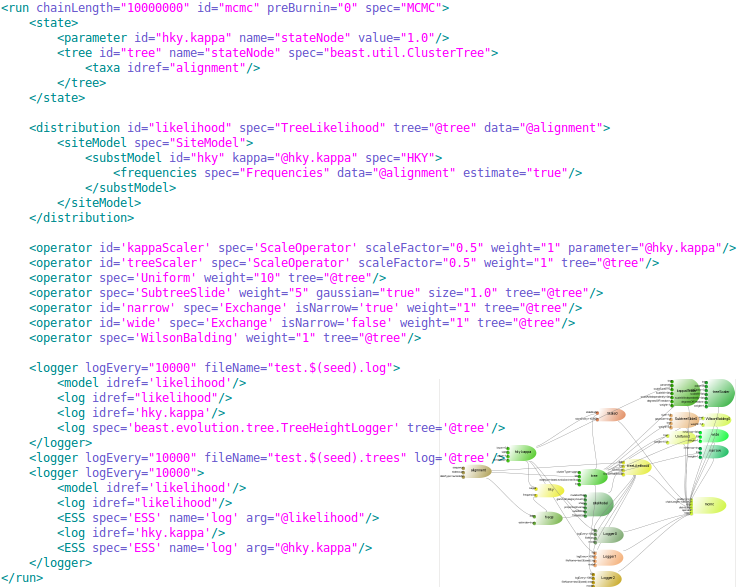
\includegraphics[width=0.95\textwidth]{xml4.png}
\end{frame}


\begin{frame}[containsverbatim]{XML}
XMLParser produces semi sensible parser error messages:

{\tiny
\begin{verbatim}

Error 124 parsing the xml input file

This plugin (treeLikelihood) has no input with 
name xxx. Choose one of these inputs: data,tree,
siteModel,branchRateModel,useAmbiguities

Error detected about here:
  <beast>
      <run id='mcmc' spec='MCMC'>
          <distribution id='posterior' spec='CompoundDistribution'>
              <distribution id='treeLikelihood' spec='TreeLikelihood'>
\end{verbatim}
}

and

{\tiny
\begin{verbatim}
Error 122 parsing the xml input file

Cannot create class: CompoundDistibution. Class could not be found. 
Did you mean beast.core.util.CompoundDistribution?

Error detected about here:
  <beast>
      <run id='mcmc' spec='MCMC'>
          <distribution id='posterior' spec='CompoundDistibution'>

\end{verbatim}
}
\end{frame}



\section{Add-ons}
\begin{frame}{Add-ons}
A BEAST 2 add-on is a library based on BEAST 2\vskip1cm

Why add-ons:
\begin{itemize}
\item Making work easier citable
\item Making the core easier to learn -- it's a lot smaller / cleaner
\item Separating out stable / experimental code / dead code
\item ...
\end{itemize}

\end{frame}

\begin{frame}{Add-ons}

\begin{itemize}
\item SnAP - multi-species coalescent for SNP and AFLP data
\url{http://code.google.com/p/snap-mcmc/}
\item beastii - utilities, Peter Will's AARS substitution model
\url{http://code.google.com/p/beastii/}
\item Subst-BMA - Bayes model averaging over subst. models
\url{http://code.google.com/p/subst-bma/}
\item EBSP/*BEAST - Joseph's thesis work
\item Experimental phylogeography
\item David Welch's Prevalence/SI-likelihood
\item Sibon's MCMC monitoring thing
\item ...
\end{itemize}
\end{frame}

\begin{frame}{What makes an Add-on}

\begin{itemize}
\item A jar file that contains the code
\item A jar file with the source
\item Example XML files
\item Documentation
\item A BEAUti 2 template
\end{itemize}\vskip0.5cm

Recommended directory structure:\\
\begin{tabular}{ll}
{\color{blue}\tt myAddOn/../beast2} &Beast 2 files\\
{\color{blue}\tt myAddOn/src} &source files\\
{\color{blue}\tt myAddOn/examples} &XML examples\\
{\color{blue}\tt myAddOn/build} &class files\\
{\color{blue}\tt myAddOn/build/dist} &jar files\\
{\color{black}\tt myAddOn/lib} &libraries used (if any)\\
{\color{black}\tt myAddOn/doc} &documentation\\
{\color{black}\tt myAddOn/templates} &BEAUti templates (optional)
\end{tabular}

\end{frame}

\begin{frame}{Setting up an Add-on}
Checkout BEAST 2 code, available at
\url{http://code.google.com/p/beast2}\vskip0.5cm

Setting up an add-on in Intellij, basic steps
\begin{itemize}
\item Make a project containing BEAST 2
\item Create new module, e.g. called MyAddOn
\item Create module dependency of MyAddOn on BEAST 2
\end{itemize}
see SDK documentation for more details.\vskip0.5cm

Setting up an add-on in Eclipse, basic steps
\begin{itemize}
\item Make a project containing BEAST 2
\item Create new project, e.g. called MyAddOn
\item Add BEAST 2 to the Java build path of MyAddOn
\end{itemize}
see SDK documentation for more details.\vskip0.5cm

Setting up an add-on in Hudson (for automatic regression testing): ask Walter
\end{frame}

\begin{frame}{Distributing Add-ons}

\begin{itemize}
\item Create Add-on files containing add-on classes only
\item Put on a web-site
\item Download to \$BEAST\_HOME/beastlib
\item It will be picked up from there when running BeastMCMC or BEAUti
\end{itemize}

Future work: automate this process, provide catalogue, GUI, etc.

\end{frame}


\section{Applications}

\begin{frame}{BEAUti 2: replacement of BEAUti 1}
\includegraphics[width=\textwidth]{BEAUti.png}

More about BEAUti in Part III
\end{frame}


\begin{frame}{Model builder: GUI for graphical manipulation of Plugins}
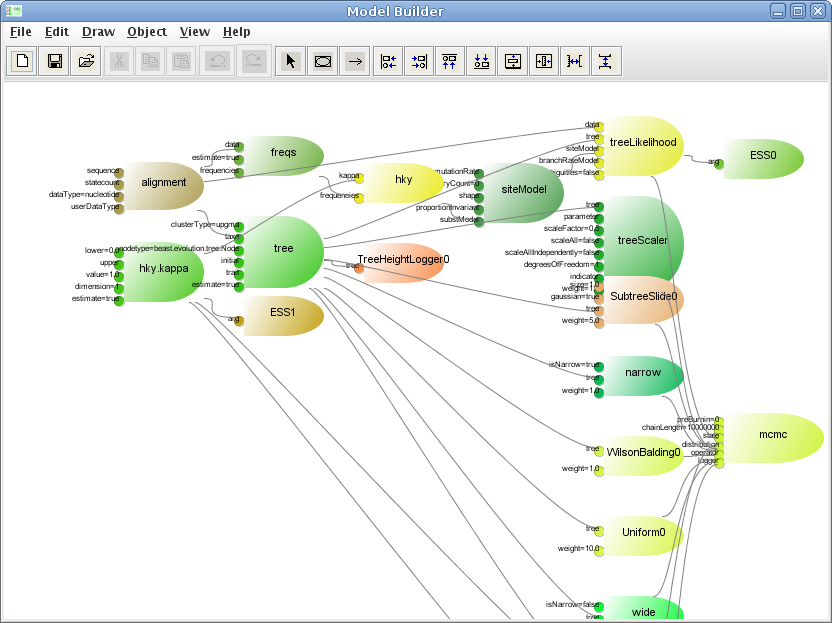
\includegraphics[width=\textwidth]{modelbuilder.png}

In development...
\end{frame}

\begin{frame}{Spreadsheet: calculates partial results on the fly}
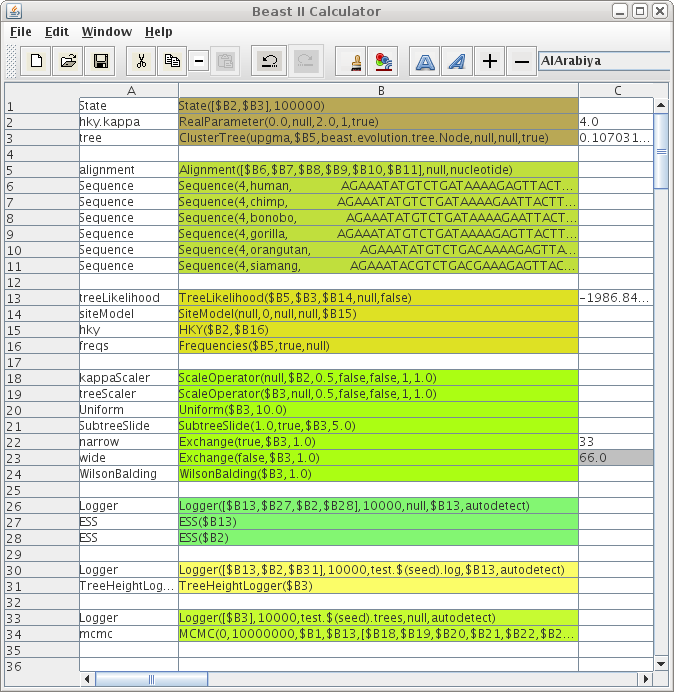
\includegraphics[width=0.8\textwidth]{spreadsheet.png}

In development...
\end{frame}

\begin{frame}{Documentation}
XML documentation provided through

\begin{itemize}
\item @Description annotation on plug in
\item Tooltip text on inputs
\item getCitation method
\item Input validation rules
\end{itemize}

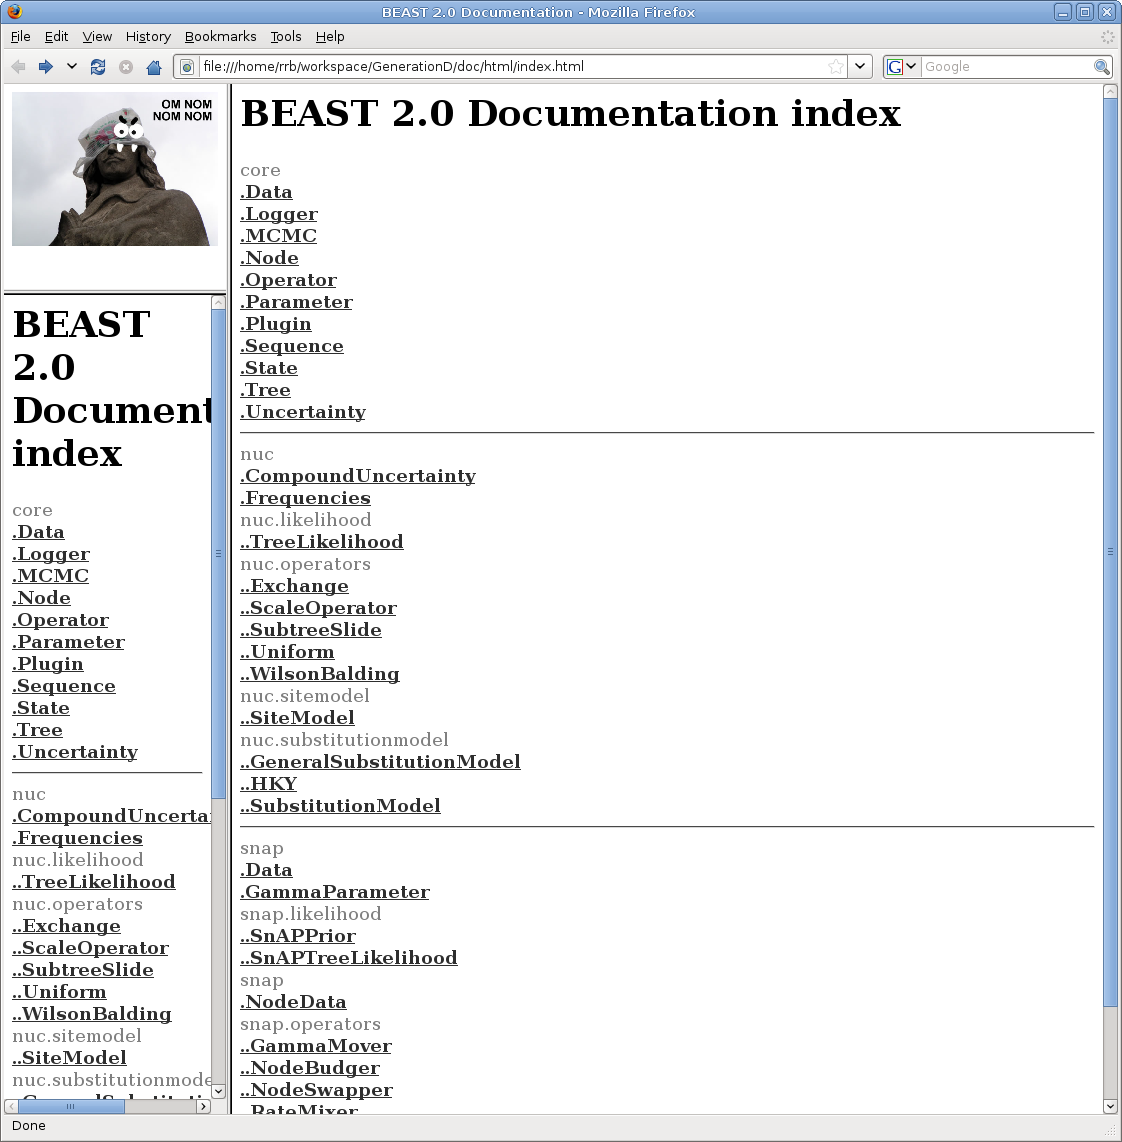
\includegraphics[width=\textwidth]{beastdoc0.png}

\end{frame}


\begin{frame}{Other}
o Sequence generator, for simulation studies\\\vskip0.5cm
o Sequence with XML merging through BEAUti, handy for scripting\\\vskip0.5cm
o XMLParser to BEAUtify XML\\\vskip0.5cm
o Alignment viewer: navigate an alignment\\\vskip0.5cm
o Log analyser: prints statistics of a trace log from command line \\\vskip0.5cm
%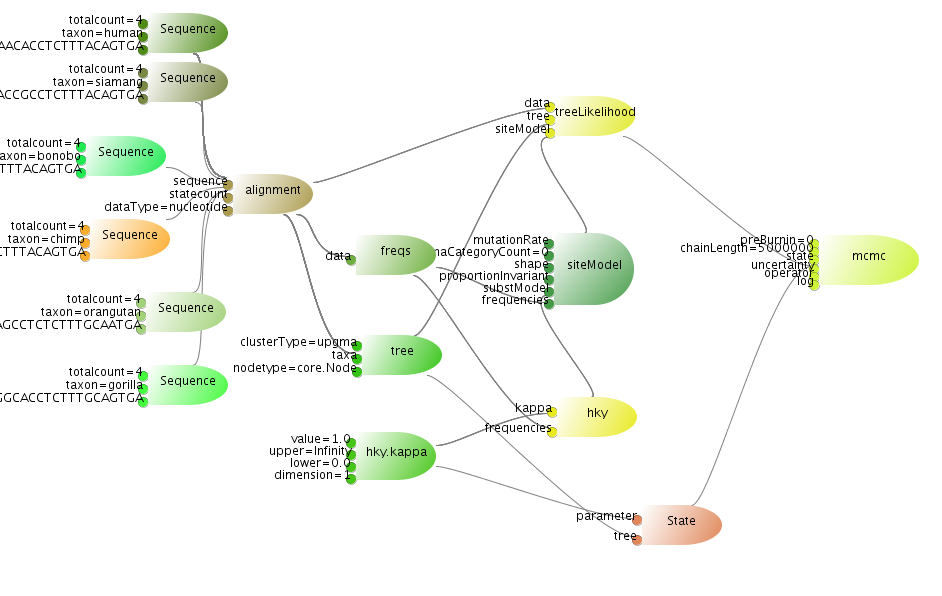
\includegraphics[width=\textwidth]{hkymodel2.png}
\end{frame}




\begin{frame}[containsverbatim]
{BEAST 2.0}

\begin{lstlisting}[language=java]
~> java beast.app.BeastMCMC

Usage: BeastMCMC [options] <Beast.xml>
where <Beast.xml> the name of a file specifying a BEAST run
and the following options are allowed:
-resume : read state that was stored at the end of the last run from file and append log file
-overwrite : overwrite existing log files (if any). By default, existing files will not be overwritten.
-seed [<int>|random] : sets random number seed (default 127), or picks a random seed
-threads <int> : sets number of threads (default 1)
-beastlib <path> : Colon separated list of directories. All jar files in the path are loaded. (default 'beastlib')
\end{lstlisting}
\end{frame}

\fi



\if \part 3

\begin{frame}[containsverbatim]{What is BEAUti 2}

A GUI for manipulating BEAST 2 specifications\vskip0.5cm

Features:
\begin{itemize}
\item Read/write XML specifications
\item Customizable GUI through templates
\item Interactive validation of specification
\item Automatically picks up plug-ins from Add-ons
\item Batch merging of alignments to XML specifications
\end{itemize}
\end{frame}


\section{BEAUti 2: A walk through}

\begin{frame}[containsverbatim]{Start up}
\includegraphics[width=0.6\textwidth]{BEAUti0.png}

Before editing anything, BEAUti needs to know either alignments and template OR existing file.
\end{frame}
\begin{frame}[containsverbatim]{Start up: select alignments}
\includegraphics[width=0.6\textwidth]{BEAUti1.png}

Select one or more alignments\\
Select an analysis template
\end{frame}
\begin{frame}[containsverbatim]{Start up: select existing file}
\includegraphics[width=0.6\textwidth]{BEAUti2.png}
\end{frame}
\begin{frame}[containsverbatim]{Edit parameters}
\includegraphics[width=0.8\textwidth]{BEAUti5.png}

Familiar panel based user interface for configuring specification
\end{frame}
\begin{frame}[containsverbatim]{Flow}
\includegraphics[width=1\textwidth]{BEAUti3.png}

No new alignment selection once editing is started
\end{frame}

\begin{frame}[containsverbatim]{Start up}
\begin{lstlisting}[language=java]
java beast.app.BEAUti.BEAUti [options]
where options can be one of the following:
-template [template file]
-nex [nexus data file]
-xmldat [beast xml file]
-xml [beast file]
-out [output file name]
-exitaction [writexml|usetemplate|usexml]
\end{lstlisting}

Select proper command line functions to short cut the flow\\
Multiple alignment files allowed\\
Batch merging of alignment with template

\end{frame}

\begin{frame}[containsverbatim]{Start up: another template}
\includegraphics[width=0.8\textwidth]{BEAUti4.png}

Template for SNP and AFLP analysis\\
Customised labels, template button invisible
\end{frame}
\begin{frame}[containsverbatim]{Edit: another template}
\includegraphics[width=0.8\textwidth]{BEAUti7.png}

Custom menu\\
Only subset of panels used
\end{frame}

\begin{frame}[containsverbatim]{Spot the differences}
\includegraphics[width=\textwidth]{BEAUti6.png}

Customized labels\\
Button visibility
\end{frame}
\begin{frame}[containsverbatim]{Spot the differences}
\includegraphics[width=\textwidth]{BEAUti8.png}

Customized menus: visibility and label names\\
Customized panels\\

\end{frame}

\begin{frame}[containsverbatim]{Configurable}
\includegraphics[width=0.6\textwidth]{BEAUti9.png}

A: Partitionable or not\\
B: Custom behaviour: gamma shape only shown when categories at least 2\\
C: Expand inputs of a plugin\\
D: Hide irrelevant inputs
\end{frame}


\begin{frame}[containsverbatim]{What BEAUti does}

\begin{itemize}
\item Contain a large number of Plugin objects, to ensure a somewhat sensible set of choices\\
\item User changes link in the model graph
\includegraphics[width=0.8\textwidth]{BEAUti10.png}\\
\item User changes values of primitive (String, Integer, Boolean, Double) inputs\\
\item Automatically update links, e.g. Operator to MCMC\vskip0.5cm
\end{itemize}

Expert mode allows creation of new Plugin object, but the user is on its own as far as validation is concerned

\end{frame}

\section{BEAUti 2 Templates}

\begin{frame}[containsverbatim]{How to configure BEAUti}

1: XML template\vskip1cm

2: Custom InputEditor classes
\end{frame}


\begin{frame}[containsverbatim]{BEAUti templates}

A BEAUti template is an XML specification with extra features
\begin{itemize}
\item {\tt <plate var='n' range='#alignments'>} 'macros'
\item {\tt <data id="#alignments"/>} for merging alignments
\item {\tt <mergepoint>}/{\tt <mergewith>} for merging sub-templates
\item {\tt <BEAUticonfig spec='beast.app.BEAUti.BEAUtiConfig'>} for customizing GUI components
\end{itemize}\vskip0.5cm


Main-templates define type of analysis, e.g. vanilla alignment analysis, *BEAST, Snap\vskip0.5cm

Sub-templates define parts that go anywhere in a main template, e.g. substitution or branch rate models.


\end{frame}


\begin{frame}[containsverbatim]{{\tt plate} element in templates}

Plate behaves like a macro

{\tt<plate var='n' range='a,b,c'>\\
 <input id='\$(n)'/>\\
</plate>}

is interpreted as\\
{\tt<input id='a'/>\\
<input id='b'/>\\
<input id='c'/>\\
}
\vskip0.5cm

For example{\small

\begin{verbatim}<plate var='n' range='#alignments'>
        <input spec='HKY' id='$(n).hky'>
            <kappa idref='$(n).hky.kappa'/>
            <frequencies id='$(n).freqs' spec='Frequencies'>
                <data idref='$(n)'/>
            </frequencies>
        </input>
</plate>\end{verbatim}
}

\end{frame}

\begin{frame}[containsverbatim]{Merging alignments}

Single alignment merging:\vskip0.5cm

{\tt <data id="\#alignments"/>}\vskip0.5cm

becomes\vskip0.5cm

\includegraphics[width=\textwidth]{BEAUtiseq.png}\vskip0.5cm

and everywhere in the template {\tt \#alignments} becomes {\tt dna}

\end{frame}

\begin{frame}[containsverbatim]{Merging alignments}

Multi alignment merging:\vskip0.5cm

{\tt <data id="\#alignments"/>}\vskip0.5cm

becomes\vskip0.5cm

\includegraphics[width=\textwidth]{BEAUtiseq2.png}\vskip0.5cm

and everywhere in the template {\tt \#alignments} becomes {\tt 26,29}

\end{frame}

\begin{frame}[containsverbatim]{{\tt mergepoint} and {\tt mergewith} elements}

Main templates define {\tt mergepoint}s with ids\vskip0.5cm

Sub-templates define {\tt mergwith} and point to the {\tt mergepoint}s in main template\vskip0.5cm

Typical usage of sub-templates
\begin{itemize}
\item specify a new substitution model,
\item specify prior distributions on parameters of the model
\item specify operators on parameters of the model
\end{itemize}
\end{frame}

\begin{frame}[containsverbatim]{{\tt mergepoint} and {\tt mergewith} Example}

Main-template
\begin{verbatim}
    <plate var='n' range='#alignments'>
        <mergepoint id='substitutionmodel'/>
    </plate>
\end{verbatim}


Sub-template
\begin{verbatim}
    <mergewith point='substitutionmodel'>
        <input spec='WAG' id='$(n).WAG'/>
    </mergewith>
\end{verbatim}

Interpretation of main template

\begin{verbatim}
    <plate var='n' range='#alignments'>
        <input spec='WAG' id='$(n).WAG'/>
    </plate>
\end{verbatim}


\end{frame}

\begin{frame}[containsverbatim]{Configuring BEAUti GUI}
In template:

{\tt <BEAUticonfig spec='beast.app.BEAUti.BEAUtiConfig'>} 

for customizing 
\begin{itemize}
\item which panels are shown at start up
\item which menus are visible in menubar
\item which buttons are visible
\item which inputs are hidden
\item which inputs are expanded inline
\item which labels are used
\end{itemize}

See files in {\tt beast2/templates} directory for details
\end{frame}

\section{BEAUti 2 Custom GUI}

\begin{frame}[containsverbatim]{Developing custom GUI components}

From a developers view: everything is a Plugin\vskip0.5cm

BEAUti is a tool for \\
\begin{itemize}
\item connecting inputs with Plugins\\
\item configuring inputs\vskip0.5cm
\end{itemize}

In BEAUti, a panel for a Plugins shows a list of InputEditors.\vskip0.5cm

To create customized behaviour for inputs of specific types, 
override InputEditor
\end{frame}

\begin{frame}[containsverbatim]{InputEditor}


BEAUti uses the input editor associated with the in type of the InputEditor\vskip0.5cm


\begin{lstlisting}[language=java]
public class MyInputEditor extends InputEditor {

    /** tell the type of input that this Input 
        Editor applies to **/
	@Override
    public Class<?> type() {
        return MyPlugin.class;
    }

    /** custom implementation **/

} 
\end{lstlisting}

See code for gory details of custom implementation possibilities\vskip0.5cm

{\tt beast.app.BEAUti} packages for examples

\end{frame}


\begin{frame}[containsverbatim]{ListInputEditor}

Dealing with list of inputs: extend ListInputEditor
and implement {\tt type()} and {\tt baseType()}

\begin{lstlisting}[language=java]
public class MyInputEditor extends ListInputEditor {

    /** tell the type of input that this Input 
        Editor applies to **/
	@Override
	public Class<?> type() {
		return List.class;
	}
	@Override
	public Class<?> baseType() {
		return Operator.class;
	}

    /** custom implementation **/

} 
\end{lstlisting}

\end{frame}


\begin{frame}[containsverbatim]{All done!}

Go forth and develop new Plugins \\and BEAUti templates now!\vskip1cm

\begin{center}
\includegraphics{../../src/beast/app/draw/icons/beast.png}
\end{center}
\end{frame}

\fi

\end{document}



